%Tex root = ProbabilitàEStatistica.tex

\chapter{Probabilità}

\Definizione{probabilità classica}{
La \textbf{probabilità classica} si calcola come:
\begin{equation*}
    \boldsymbol{\mathrm{P_{classica}} = \frac{\mathrm{n\textsuperscript{o} \ casi \ favorevoli}}{\mathrm{n\textsuperscript{o} \ casi \ possibili}}}
\end{equation*}
}

\esempio{lancio del dado}{
\textbf{Qual'è la probabilità di ottenere 4 lanciando un dado da 6 faccie?}
\begin{equation*}
    \mathrm{P} = \frac{1}{6}
\end{equation*}
}

\esempio{lancio della moneta}{
\textbf{Qual'è la probabilità di ottenere testa lanciando una moneta}
\begin{equation*}
    \mathrm{P} = \frac{1}{2}
\end{equation*}
}

La definizione di probabilità classica, però, vale solo quando gli eventi sono \textcolor{viola}{\textbf{equiprobabilit}} e, inoltre, presuppone un numero finiti di casi possibili.

\section{Probabilità non condizionata}

\Definizione{eventi (in)compatibili}{
Due eventi si dicono \textbf{compatibili} se possono accadere contemporaneamente.

\noindent\rule{\textwidth}{0.4pt}

\medskip
Due eventi si dicono \textbf{incompatibili} se \textcolor{red}{\textbf{non}} possono accadere contemporaneamente.
}

\vario{Teorema della probabilità totale}{
Siano $\mathrm{A}$ e $\mathrm{B}$ due eventi diversi tra loro:
\begin{equation*}
    \boldsymbol{\mathrm{P(A \cup B)} = \mathrm{P(A)} + \mathrm{P(B)} - \mathrm{P(A \cap B)}}
\end{equation*}

\begin{itemize}[label=$\triangleright$]
    \item $\mathrm{P(A \cup B)}$: probabilità che si verifichi $\mathrm{A}$ o $\mathrm{B}$ (almeno uno dei due eventi)
    \smallskip
    \item $\mathrm{P(A \cap B)}$: probabilità che si verifichi sia $\mathrm{A}$ che $\mathrm{B}$ (contemporaneamente)
\end{itemize}
}

Nel caso in cui i due eventi sono incompatibili, allora $\mathrm{P(A \cap B)} = 0$.

\esempio{lancio del dado}{
\textbf{Qual'è la probabilità che lanciando un dado esca come risultato 3 oppure 4?}

\smallskip
$\Rightarrow$ gli eventi A (esce 3) e B (esce 4) sono due eventi incompatibili, perchè non può uscire 3 e contemporaneamente 4.

\smallskip
Di conseguenza:
\[
    \begin{aligned}
    \mathrm{P} &= \mathrm{P(A)} + \mathrm{P(B)} - \cancel{\mathrm{P(A \cap B)}}\\
    &= \frac{1}{6} + \frac{1}{6} - 0\\
    &= \frac{1}{3}
    \end{aligned}
\]
}

\esempio{lancio del dado}{
\textbf{Qual'è la probabilità che lanciando un dado esca un numero pari o un multiplo di 3?}

\smallskip
$\Rightarrow$ gli eventi A (esce un numero pari) e B (esce un numero multiplo di 3) sono due eventi compatibili, perchè:
\begin{itemize}[label=$\triangleright$]
    \item numeri pari: $\{2, 4, 6\}$
    \item multipli di 3: $\{3, 6\}$
\end{itemize}

\smallskip
Di conseguenza:
\[
    \begin{aligned}
    \mathrm{P} &= \mathrm{P(A)} + \mathrm{P(B)} - \mathrm{P(A \cap B)}\\
    &= \frac{3}{6} + \frac{2}{6} - \frac{1}{6}\\
    &= \frac{2}{3}
    \end{aligned}
\]
}

Il teorema della probabilità totale si può generalizzare anche quando si considerano 3 o più eventi.

\section{Probabilità condizionata}

    

\Definizione{eventi (in)dipendenti}{
Due eventi si dicono \textbf{indipendenti} se il fatto che si verifichi (o meno) il primo \textcolor{red}{\textbf{non}}, altera la probabilità che si verifichi il secondo.

\noindent\rule{\textwidth}{0.4pt}

\medskip
Due eventi si dicono \textbf{dipendenti} se il fatto che si verifichi (o meno) il primo, altera la probabilità che si verifichi il secondo.
}

\textbf{Qual'è la probabilità che lanciando contemporanemente un dado e una moneta si ottengono un 4 e una testa?}
\[
    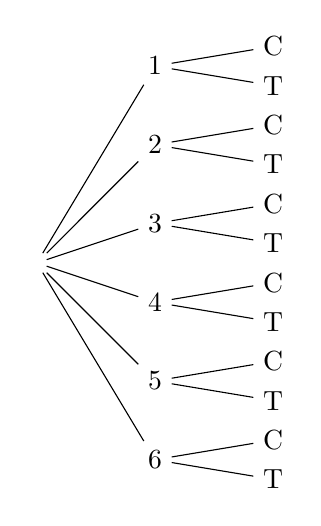
\begin{tikzpicture}[
    level 1/.style={sibling distance=1cm},
    level 2/.style={sibling distance=0.5cm},
    grow=right, 
    sloped
    ]
    \node {}
        child {node {6}
        child {node {T}}
        child {node {C}}
        }
        child {node {5}
        child {node {T}}
        child {node {C}}
        }
        child {node {4}
        child {node {T}}
        child {node {C}}
        }
        child {node {3}
        child {node {T}}
        child {node {C}}
        }
        child {node {2}
        child {node {T}}
        child {node {C}}
        }
        child {node {1}
        child {node {T}}
        child {node {C}}
        };
    \end{tikzpicture}
\]

I due eventi sono indipendenti:
\begin{equation*}
    \mathrm{P} = \frac{1}{6} \cdot \frac{1}{2} = \frac{1}{12}
\end{equation*}

\vario{Eventi indipendenti}{
Se $\mathrm{A}$ e $\mathrm{B}$ sono due eventi indipendenti:
\begin{equation*}
    \boldsymbol{\mathrm{P(A \cap B)} = \mathrm{P(A)} \cdot \mathrm{P(B)}}
\end{equation*}
}

\textbf{In una classe ci sono 20 alunni (12 femmine e 8 maschi): se la prof ne sceglie 2 random, qual'è la probabilità che scelga due ragazze?}

I due eventi sono dipendenti:
\begin{equation*}
\mathrm{P} = \frac{\binom{12}{2}}{\binom{20}{2}} = \frac{\frac{\cancel{12!}}{\cancel{2!} \cdot \cancel{10!}}}{\frac{\cancel{20!}}{\cancel{2!} \cdot \cancel{18!}}} = \frac{12 \cdot 11}{20 \cdot 19}
\end{equation*}

\begin{itemize}[label=$\Rightarrow$]
\item $\frac{12}{20}$: probabilità di scegliere una ragazza
\medskip
\item $\frac{11}{19}$: probabilità di scegliere una ragazza, sapendo che ne ho già scelta una prima
\end{itemize}

\vario{Eventi dipendenti}{
Se $\mathrm{A}$ e $\mathrm{B}$ sono due eventi dipendenti:
\begin{equation*}
    \boldsymbol{\mathrm{P(A \cap B) = P(A) \cdot P(B \mid A)}}
\end{equation*}
}